\documentclass[a4paper,11pt]{book}
\usepackage[T1]{fontenc}
\usepackage[utf8]{inputenc}
\usepackage{lmodern}
\usepackage{titling}
\renewcommand\maketitlehooka{\null\mbox{}\vfill}
\renewcommand\maketitlehookd{\vfill\null}

\usepackage{hyperref}
\usepackage{graphicx}
\usepackage[english]{babel}
\usepackage{verbatim}
\usepackage{tikz}
\usepackage{ifthen}
\usepackage{xstring}
\usepackage{calc}
\usepackage{pgfopts}


\newenvironment{dedication}
{
   \cleardoublepage
   \thispagestyle{empty}
   \vspace*{\stretch{1}}
   \hfill\begin{minipage}[t]{0.66\textwidth}
   \raggedright
}
{
   \end{minipage}
   \vspace*{\stretch{3}}
   \clearpage
}


\makeatletter
\renewcommand{\@chapapp}{}% Not necessary...
\newenvironment{chapquote}[2][2em]
  {\setlength{\@tempdima}{#1}%
   \def\chapquote@author{#2}%
   \parshape 1 \@tempdima \dimexpr\textwidth-2\@tempdima\relax%
   \itshape}
  {\par\normalfont\hfill--\ \chapquote@author\hspace*{\@tempdima}\par\bigskip}
\makeatother


\begin{document}
\begin{figure}[htp]
\centering
\includegraphics[width=12cm]{images/logo}
\end{figure}
\chapter{User manual}
\section{Dashboard}
\begin{figure}[htp]
\centering
\includegraphics[width=10cm]{images/dashboard}
\includegraphics[width=10cm]{images/topicdash}
\caption{Bam dashboard}
\label{fig:lion}
\end{figure}
\subsection{Top section dashboard}
The top of the dashboard gives the user access to the following information:
\begin{itemize}
    \item A link to the calendar of the trainer’s current batch.
    \item Personal information about the trainer.
    \item Information about the batch.
    \item The progress of the batch, measured in number of days completed and number of subtopics completed
\end{itemize}
\subsection{Bottom section dashboard}
The bottom of the dashboard gives the user access to the following information:
\begin{itemize}
    \item A link to the calendar of the trainer’s current batch.
\end{itemize}

\begin{figure}[htp]
\centering
\includegraphics[width=10cm]{images/Batchview}
\caption{All Batches}
\label{fig:lion}
\end{figure}

\subsection{All Batches}
The All Batches tab gives the user access to the following functionality:

\begin{itemize}
    \item Search for keywords matching fields in the all batches table using the search bar in the top right corner.
    \item View information about all batches, including batch name, trainer, batch type, and the start and end date of the batch
\end{itemize}

\subsection{My Batch}
The My Batches tab gives the user access to the following information:

\begin{figure}[htp]
\centering
\includegraphics[width=10cm]{images/myBatch}
\caption{All Batches}
\label{fig:lion}
\end{figure}

\begin{itemize}
    \item Current Batches – Information about the batch(es) currently in progress that a trainer is responsible for
    \item Past Batches – Information about the batch(es) that have been completed that a trainer was responsible for
    \item Future Batches – Information about the batches that the trainer will be responsible for in the future
\end{itemize}

\subsection{Calender}
The Calendar grants the user the following functionality:
\begin{figure}[htp]
\centering
\includegraphics[width=10cm]{images/calendarView}
\caption{Calender view}
\label{fig:lion}
\end{figure}

\begin{itemize}
    \item View the schedule of subtopics to be covered on a certain date for a batch
    \item Add a subtopic to the calendar by:
    \begin{itemize}
        \item Selecting the topic the subtopic you wish to add is located.
        \item Choose the subtopic to add to the date.
        \item Select the date to cover that subtopic.
        \item Select “Add to Calendar”.
    \end{itemize}
        
    \item Add a subtopic to the calendar by:
    \begin{itemize}
        \item Selecting the topic the subtopic you wish to add is located.
        \item Dragging the subtopic to wish to add to the date on the calendar.
    \end{itemize}
        
    \item Change the status of a subtopic by:
    \begin{itemize}
        \item Clicking on the subtopic you wish to change the status of in the calendar until the status you wish to give it is reached.
    \end{itemize}
    \item Change the date a subtopic is covered by:
    \begin{itemize}
        \item Dragging the subtopic to the new date you wish to cover the subtopic.
    \end{itemize}
    \item Remove a subtopic from the schedule by:
    \begin{itemize}
        \item Dragging the subtopic you wish to remove from the schedule to the trash can icon.
    \end{itemize}
\end{itemize}
\subsection{Curriculum Editor}
The Curriculum Editor gives the user the following functionality:
\begin{figure}[htp]
\centering
\includegraphics[width=10cm]{images/curriculumView}
\caption{Curriculum Editor}
\label{fig:lion}
\end{figure}

\begin{itemize}
    \item Export Curriculum – Exports an Excel file containing the curriculum plan based on the current curriculum in the editor
    \item Populate my Calendar – Populates the calendar for the current batch with the current curriculum in the editor
    \item Delete Curriculum Version – Delete the curriculum version by:
    \begin{itemize}
        \item Clicking the trash can icon to the top right of the Curriculum Editor when the version you wish to delete is displayed.
        \item Confirm that you want to delete that version of the curriculum.
    \end{itemize}
\end{itemize}
The Course Structures tab side menu gives the user the following functionality:
\begin{itemize}
    \item Add New Curriculum Label – Allows the user to create a new curriculum label that can maintain one or more curriculum versions by:
    \begin{itemize}
        \item Clicking “Add New Curriculum”.
        \item Entering the name of the label into the text box.
    \end{itemize}
    \item Add New Curriculum – Allows the user to create a new version of a curriculum under an existing label by:
    \begin{itemize}
        \item Clicking the “plus” symbol next to the label you wish to create a new curriculum version for.
        \item Populating each week inside of the newly created curriculum version template.
    \end{itemize}
\end{itemize}

\subsubsection{Topic Pool}
The Topic Pool tab side menu gives the user the following functionality:

\begin{figure}[htp]
\centering
\includegraphics[width=10cm]{images/TopicView}
\caption{Topic Pool}
\label{fig:lion}
\end{figure}

\begin{itemize}
    \item Add New Topic – The user can create a new topic for the topic pool by:
    \begin{itemize}
        \item Clicking “Add New Topic”.
        \item Entering the name of the new topic into the text box.
    \end{itemize}
    \item Add New Subtopic – The user can create a new subtopic for a topic by:
    \begin{itemize}
        \item Clicking the “plus” icon next to the topic you wish to add a new subtopic to.
        \item Entering the name of the new subtopic into the text box.
    \end{itemize}
    \item Search Topics – Allows you to search for subtopics by name.
\end{itemize}
\subsection{Objectives Manager}
The Objectives Manager’s Subtopics Completion Chart gives the user the following information:

\begin{figure}[htp]
\centering
\includegraphics[width=10cm]{images/Objective}
\caption{Objectives Manager}
\label{fig:lion}
\end{figure}


\begin{itemize}
    \item A pie chart showing the number of batches that completed less than x percent of subtopics and the number of batches that completed x percent or more subtopics.
    \item An overall progress table for each active batch, showing the batch name, the trainer, number of missed and completed sub tasks, and the current week the batch is in
\end{itemize}

\begin{figure}[htp]
\centering
\includegraphics[width=10cm]{images/WeeklyObj}
\caption{Weekly Progress}
\label{fig:lion}
\end{figure}

The Objectives Manager’s Weekly Progress Chart gives the user the following information:
\begin{itemize}
    \item A bar graph showing the percentage of subtopics completed for each week of a batch.
\end{itemize}

\chapter{Overview}
\section{BAM}
BAM is Revature's batch management platform for recording and retrieving batch information. It is built with a cutting edge, micro service architecture to allow for modularity, system resilience, and fast development. It’s infrastructure services include a circuit breaking metric display, multiple discovery services for heartbeat monitoring, a configuration server for business service backups, and an API gateway that handles redirecting requests to different business services.

\section{Infrastructure}
\subsection{Discovery Service}
Discovery services are used to monitor business micro-services through the use of heart beats. This application utilizes Eureka to send heart beats out on timed intervals. This helps reduce API calls to micro-services that are no longer operational.

\subsection{Configuration Service}
Configuration Service used to apply a uniform configuration across specified micro-services. This application uses Configuration Server to provide configurations to any backup services that are needed to be spun up. It helps reduce repeated configuration files across micro-service applications.

\subsection{API Gateway}
API gateways are used to provide a single endpoint for client’s to access and it can apply filters across data. This application uses Zuul Netflix dependency to redirect client requests to different online business micro-services. It helps direct traffic throughout the system and allows for dynamic trafficking with the help of the circuit breaker.

\subsection{Circuit Breaking Service}
Circuit breaking is used to improve BAM’s resiliency. This application uses Hystrix dashboard and Hystrix circuit breaker to handle errors with fallback methods. The Hystrix dashboard allows easy monitoring of all business service clusters and their circuit breakers.

\subsection{Business Services}
Business services are the micro-services that handle any application specific operations. In BAM, these business services consist of: User micro-service, Batch micro-service, Curriculum micro-service, and Topic micro-service.Each of these micro-services persist data and also expose internal endpoints for any other business micro-service to request resources.

\subsection{Infrastructure Design}
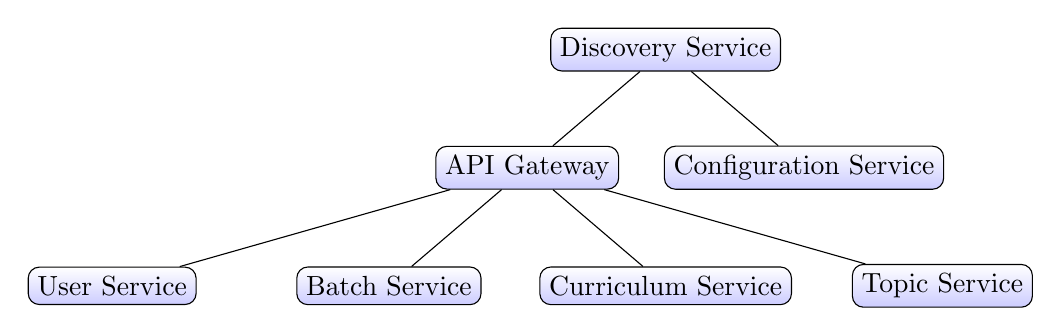
\begin{tikzpicture}[sibling distance=10em,
  every node/.style = {shape=rectangle, rounded corners,
    draw, align=center,
    top color=white, bottom color=blue!20}]]
  \node {Discovery Service}
    child { node {API Gateway}
        child { node {User Service}} 
        child { node {Batch Service}}
        child { node {Curriculum Service}}
        child { node {Topic Service}}}
    child { node {Configuration Service}};
\end{tikzpicture}

\chapter{States}
\begin{figure}[htp]
\centering
\includegraphics[width=15cm]{images/Overall}
\caption{State Diagram}
\label{fig:lion}
\end{figure}

\begin{figure}[htp]
\centering
\includegraphics[width=15cm]{images/internalDocs}
\caption{Internal Connection}
\label{fig:lion}
\end{figure}


\chapter{System Requirements}
\begin{itemize}
    \item Java 8
    \item Maven
    \item Spring boot starter 1.5 +
    \item Angular 4 +
    \item Angular Cli 1.4 +
    \item CLI tool
\end{itemize}
\chapter{Curriculum Service}
\section{Abstract}
The curriculum micro-service is crucial to our design as well as the original monoliths. In the monolith, the curriculum model contained information from curriculum service and the topic service. Each of those services retrieved data from their respective repositories for the curriculum model. When converting the monolith to a micro-service architecture, the micro-services are determined by the model and the internal service communication is handled via REST templates. The services in the original monolith are now basically the internal service communication that is going on in between the business services. We chose to keep many of the same endpoints as the original monolith to reduce the necessary changes in the front end application Janus.


\section{Service Architecture}

\begin{figure}[htp]
\centering
\includegraphics[width=18cm]{images/curriculum-package}
\includegraphics[width=18cm]{images/curriculum-class}
\caption{Curriculum Service Infrastructure}
\label{fig:lion}
\end{figure}


\begin{figure}[htp]
\centering
\includegraphics[width=5cm]{images/controller}
\includegraphics[width=5cm]{images/curriculumRepo}
\includegraphics[width=5cm]{images/curriculumBean}
\includegraphics[width=5cm]{images/curriculumService}
\caption{Curriculum Service Hierarchy}
\label{fig:lion}
\end{figure}
\chapter{Batch Service}
\section{Abstract}
The batch micro-service is a major component of this micro-service system. It communicates with the user micro-service which gives individual details about each user in the system. They are tied together with keys but stored individually in completely different databases. The batch micro-service stores batch data within the batch repository. From here, it can send data to any other micro-service that needs batch data.

\section{Batch Architecture}

\begin{figure}[htp]
\centering
\includegraphics[width=18cm]{images/batch-package}
\includegraphics[width=18cm]{images/batch-class}
\caption{Batch Service Infrastructure}
\label{fig:lion}
\end{figure}


\begin{figure}[htp]
\centering
\includegraphics[width=5cm]{images/Batchcontroller}
\includegraphics[width=5cm]{images/Batchbean}
\includegraphics[width=5cm]{images/Batchservice}
\includegraphics[width=5cm]{images/Batchrepository}
\includegraphics[width=5cm]{images/Batchexception}
\caption{Batch Service Hierarchy}
\label{fig:lion}
\end{figure}
\chapter{Topic Service}
\section{Abstract}
The topic micro-service is a large component that handles subtopics, topics, and calendar models. The original monolith had each model separate along with a controller and service for each respectively. We broke down the code from the original monolith by the models, however, the topic and subtopic models were similar enough to merge them into one micro-service. By doing this, we reduced the number of overall micro-services we had as well as the internal service communication that would have had to have taken place. The calendar model was not originally found within the monolith, so we decided to simply add the routes to the topic micro-sevice, since the calendar is only composed of a topic and subtopic.

\section{Service Architecture}

\begin{figure}[htp]
\centering
\includegraphics[width=18cm]{images/topic-package}
\includegraphics[width=18cm]{images/topic-class}
\caption{Topic Service infrastructure}
\label{fig:lion}
\end{figure}


\begin{figure}[htp]
\centering
\includegraphics[width=5cm]{images/Topiccontroller}
\includegraphics[width=5cm]{images/Topicmodel}
\includegraphics[width=5cm]{images/Topicrepository}
\includegraphics[width=5cm]{images/Topicservices}
\includegraphics[width=5cm]{images/Topicexception}
\caption{Topic Service Hierarchy}
\label{fig:lion}
\end{figure}
\chapter{User Service}
\section{Abstract}
The user micro-service is the basic component of your micro-service system. It is responsible for all user data and persisting it within a repository. Any other business service that needs user data must contact the user micro-service. The initial user model in the monolith application, receives data from a BAM user controller and stores it in the BAM user repository. In this application, we have gotten rid of the BAM user controller and the services.

\section{Service Architecture}

\begin{figure}[htp]
\centering
\includegraphics[width=18cm]{images/user-package}
\includegraphics[width=18cm]{images/user-class}
\caption{User Service Infrastructure}
\label{fig:lion}
\end{figure}


\begin{figure}[htp]
\centering
\includegraphics[width=5cm]{images/Usercontrollers}
\includegraphics[width=5cm]{images/Userbeans}
\includegraphics[width=5cm]{images/Userservice}
\includegraphics[width=5cm]{images/Userrepository}
\includegraphics[width=5cm]{images/Userexception}
\caption{User Service Hierarchy}
\label{fig:lion}
\end{figure}
\chapter{API routes}
\section{User Service API routes}
\subsection{Post request}
\begin{itemize}
  \item To drop user: /api/v2/user/drop/{userId}
  \item To update user: /api/v2/user/update/
  \item To register user: /api/v2/user/register/
  \item To remove user: /api/v2/user/remove/{userId}
  \item To add user to batch: /api/v2/user/addUserToBatch/{userId}/{batchId}
\end{itemize}

\section{Batch Service API routes}
\subsection{Get requests}
\begin{itemize}
  \item To get all batches: /api/v2/batch/all/
  \item To get list of all past batches for the trainer:   /api/v2/batch/inprogress?email={email}
  \item To get all in progress by trainer: /api/v2/batch/allinprogress?email={email}
  \item To get batch by id: /api/v2/batch/byid/{id}
  \item To get batch types: /api/v2/batch/batchtypes
  \item To get current batches: /api/v2/batch/currentbatches
  \item To get past batch by trainer email: /api/v2/batch/past?email={email}
  \item To get future batch by trainer email: /api/v2/batch/future?email={email}
\end{itemize}



\subsection{Post requests}
\begin{itemize}
 \item To update or add batch: /api/v2/batch/updatebatch
\end{itemize}

\section{Curriculum API routes}
\subsection{Get requests}
\begin{itemize}
    \item To get all curriculum: /api/v2/curriculum/all/
    \item To get curriculum by id: /api/v2/curriculum/getcurriculum/{id}
    \item To get curriculum by schedule: /api/v2/curriculum/schedule/{id}
    \item To get all topic names: /api/v2/curriculum/topicpool/
    \item To get all subtopics: /api/v2/curriculum/subtopicpool/
    \item To make master curriculum: /api/v2/curriculum/makemaster/{id}
    \item To synchronize curriculum with a batch: /api/v2/curriculum/syncbatch/{id}
\end{itemize}

\subsection{Post requests}
\begin{itemize}
    \item To add curriculum: /api/v2/curriculum/addcurriculum/
    \item To delete curriculum version: /api/v2/curriculum/deleteversion/
\end{itemize}

\section{Topic API routes}
\subsection{Get requests}
\begin{itemize}
    \item To get list of subtopics depending on what page: /api/v2/calendar/subtopicspagination/{batchId}/{pageNumber}/{pageSize}
    \item To get list of subtopics for batch: /api/v2/calendar/subtopics/{batchId}
    \item To get number of subtopics: /api/v2/calendar/getnumberofsubtopics/{batchId}
    \item To get topics by batch: /api/v2/calendar/topics/{batchId}
    \item To update status: /api/v2/calendar/statusupdate/{subtopicId}/{batchId}/{status}
\end{itemize}
\subsection{Post requests}
\begin{itemize}
    \item To update calender date: /api/v2/calendar/dateupdate/{subtopicId}/{batchId}/{date}
    \item To add topic: /api/v2/calendar/addtopics
\end{itemize}
\chapter{Challenges}
\section{Inadequate Documentation}
We started off the project without any useful documentation. We only had a SQL script from the previous batches. The code Java code itself had java docs with no concrete definition of goal of the methods and classes.
\section{Vague definition of business objectives}
There was no stakeholder for the project, we started off the project by discovering what was the application supposed to do by looking at the code and experimenting with the application itself.
\section{Revature's Given Services}
In the beginning of the project, we were handed 4 micro-services that were supposed to kick start the project. They were the core micro-services: service registry and discovery, API gateway and configuration service. They are the projects: hydra-discovery-service, hydra-gateway-service and hydra-config-service. All three of them were never tested. The configuration service was using a gitlab repository that not only didn't have suitable configuration for our micro-services but also no fall back configuration. The API gateway service was copied from another project and had all the filters an swagger classes commented out.
\section{Hardware limitations}
Starting off the project, we weren't given any help from Revature. We weren't given enough hardware (EC2 memory) to run our micro-services, or RDS databases or even the ability to create any users on the RDS database that was used in the original monolith.

\section{Front-end Issues}
The initial front-end wasn't not properly set with CORS, which means that we didn't have the ability to get data from the back-end using the given services. The front-end data models were identical to those of the back-end in the monolith, meaning that they were tightly coupled and most of the methods and models are redundantly used.
\chapter{Solutions}
\section{Documentations}
We started by writing documentation for next teams to work on this project, so they won't run into the same issues we had starting off the project. We have the document you're currently reading (Project design document) and every github repository has its wiki and milestones.

\section{Core Services}
We rewrote the core three micro-services: hydra-discovery-service, hydra-gateway-service and hydra-config-service. We also created configurations matching our micro-services names and fall back configurations. We also have setup the micro-services for containerization using Docker.

\section{Hardware Limitations}
We used our own EC2s and RDS to fill the hardware gap.

\section{Front-end solution}
We fixed the front-end models. They aren't tightly coupled anymore and we have fixed cores using HttpClient interceptors except for calendar service on the front-end because it was referenced everywhere though out the application and changing it in the time given would cause more problems than solve them. For calendar it starts having CORS problems 50 percent of the time.
\chapter{Bugs}
\section{Front-end}
The front-end services except for the interceptors need to redone to allow more flexibility and usage though out the application.
\section{Configuration service}
Because we had to use our own EC2 we couldn't make use of the configuration service. The configurations of the micro-services are tightly coupled.

\section{Dashboard service}
Because we ran through many hardware problems we couldn't configure hystrix-dashboard properly. The service hydra-dashboard needs to be redone or not used.
\chapter{Potential Improvements}
\section{Use containerization}
In micro-service architecture using containerization is ideal and save many debugging problems. Use docker swarm or PCF to configure and connect the micro-services.

\section{Use Message Queue}
In the current implementation we are using rest templates for internal service interaction. It is ideal for micro-service architecture to use streams to exchange data between services.

\section{Add channel to Hystrix dashboard}
Hystrix dashboard can used Turbine to track the health and circuit breaking of the services.

\section{Use and Add YOUR custom configuration}
Add your custom configurations to your configuration repository to match your architecture needs.

\section{Front-end}
Redo all of the services except the interceptors and everything will work flawlessly.
\end{document}